\section{第二周数值分析实验}
\subsection{第一节:插值function}
\subsubsection{直接法}
\lstinputlisting[language=matlab]{day2/Vslove.m}
\subsubsection{Lagrange法}
\lstinputlisting[language=matlab]{day2/lagrangeslove.m}
\subsection{第二节:计算实例}
\begin{ex}
	给出插值点
	$$x = (0.25, 0.3, 0.39, 0.45, 0.53, 0.66, 0.72)^T,$$  
	$$y = (0.5, 0.5477, 0.6245, 0.6708, 0.7280, 1.0254, 0.9521)^T .$$ 
	时的两种方法插值多项式表达式及对应的函数图像, 并与MATLAB拟合工具箱(cftool)进行比较.
\end{ex}
\subsubsection{直接法计算}
\lstinputlisting[language=matlab]{day2/mainvslove.m}
\subsubsection{Lagrange法计算}
\lstinputlisting[language=matlab]{day2/mainlagrange.m}
\subsubsection{结果}
\begin{figure}[H]
	\centering
	\subfloat[直接法图像]{\includegraphics[width = 0.5\linewidth]{day2/fig1.eps}}
	\hfill
	\subfloat[Lagrange法图像]{\includegraphics[width = 0.5\linewidth]{day2/fig2.eps}}
	\caption{运行结果}
	\label{fig:cj12}
\end{figure}
